\documentclass{article}

\usepackage[utf8]{inputenc}
\usepackage{caption}
\usepackage{subcaption}
\usepackage{natbib}
\usepackage{soul}
\usepackage{graphicx}
\usepackage{listings}
\usepackage[hyphens]{url}
\usepackage[table,xcdraw]{xcolor}
\usepackage{color}
\usepackage{textpos}
\usepackage{glossaries}
\usepackage{hyperref}
\usepackage{acronym}
\usepackage{verbatim}
\usepackage{amsmath}
\usepackage{amssymb}
\usepackage{comment}
\usepackage{xcolor}


\newcommand{\emailaddr}[1]{\href{mailto:#1}{\texttt{#1}}}

\begin{document}
\begin{titlepage}

  \newcommand{\HRule}{\rule{\linewidth}{0.5mm}}
  \center
  
  \textsc{\Large Department of Computer Science And Engineering}\\[0.5cm]
  
  \textsc{\Large University of Bologna}\\[0.6cm]
  
  \hrule width \hsize \kern 1mm \hrule width \hsize height 2pt 
  \vspace{0.8cm}
  { \large \bfseries DealerPro}\\[0.6cm]
  { \large \bfseries Project Proposal}\\[0.6cm]
  { \large Project Management}\\[0.6cm]
  
  
  {\bfseries{June, 2023}
  \hfill
  \bfseries{Davide Domini}}\\[0.6cm]
  
  \hrule width \hsize height 2pt \kern 1mm \hrule width \hsize height 1pt
  \vspace{0.4cm}
  
  \end{titlepage}

  \clearpage

  \tableofcontents

  \newpage
  
  \section{Executive Summary}

  \subsection{Problema}

  La gestione di una concessionaria di auto comporta una serie di processi ricorrenti e standardizzati che 
    vengono svolti dai dipendenti. Una nota concessionaria romagnola, composta da tre sedi, ha deciso di 
    rinnovare il proprio sistema informatico in quanto ritenuto ormai obsoleto.

  Il sistema attuale è stato sviluppato negli anni, in maniera frammentata, da diversi team di sviluppatori.
    Oltretutto, le attuali sedi che compongono l'azienda, in principio, erano indipendenti e sono state acquisite
    nel tempo. Questo aspetto ha portato il sistema informatico ad essere ancor più disomogeneo rendendo difficile 
    e tediosa l'integrazione dei dati delle diverse sedi.

  Tra i principali limiti del sistema attuale dunque troviamo:
  \begin{itemize}
    \item Scarsa capacità di fornire ai manager informazioni utili e aggregate per prendere decisioni strategiche;
    \item Lentezza e limitata user-experience per i dipendenti, questo causa in loro frustrazione e scarsa produttività. 
    \item Spesso i dipendenti inseriscono solo informazioni parziali o non aggiornate, questo causa una scarsa qualità dei dati;
    \item I dipendenti sono costretti a svolgere attività ripetitive e manuali che potrebbero essere automatizzate;
    \item Scarsa organizzazione interna (ad esempio, ferie e permessi dei dipendenti);
    \item Manca totalmente un sistema di gestione dei clienti per quanto riguarda gli appuntamenti periodici 
    (ad esempio, per il tagliando).
  \end{itemize}

  \subsection{Soluzione}

  DealerPro è un servizio software volto a semplificare ed automatizzare i processi della concessionaria di auto.
    Il servizio è composto da diversi moduli che si integrano tra loro, ovvero:
    \begin{itemize}
      \item \textbf{Venditori}: permette di gestire preventivi e ordini;
      \item \textbf{Clienti}: permette di gestire le esigenze dei clienti che hanno già acquistato un'auto, 
      come ad esempio: gestione degli appuntamenti ed avvisi di manutenzione obbligatoria;
      \item \textbf{Dipendenti}: permette di gestire le ferie e i permessi dei dipendenti;
      \item \textbf{Management}: permette ai manager di ottenere statistiche e report utili 
        per prendere decisioni strategiche.
    \end{itemize}

  \subsection{Impatto}
  
  Dal punto di vista della concessionaria DealerPro avrà un impatto positivo su 
    diversi aspetti, tra cui: permetterà di rinnovare e automatizzare i processi
    interni, aumenterà la soddisfazione dei dipendenti e dei clienti, 
    permetterà un monitoring più pervasivo dei risultati aziendali facilitando il 
    lavoro dei manager.

  Dal punto di vista del contraente (ovvero, il team di sviluppo) il progetto 
    permetterà di acquisire nuove competenze su un dominio di business molto importante
    al giorno d'oggi, permettendo di avere un vantaggio competitivo in futuro per lo 
    sviluppo di progetti simili.

  \subsection{Business}
  
  Per il progetto si prevede un modello di business in cui il software verrà installato in cloud. 
    Questa scelta deriva dal fatto che l'infrastruttura IT interna della concessionaria è limitata e obsoleta,
    inoltre, il cliente non è intenzionato ad effettuare investimenti consistenti in questo ambito.
    Il software verrà venduto con un modello di licenza annuale.
    Eventuali future modifiche e/o aggiunte richieste dal cliente verranno valutate e preventivate a parte.
    Si specifica che la proprietà del software rimarrà sempre del team di sviluppo che potrà riutilizzarlo tutto 
    o in parte anche per progetti futuri.



  \newpage
  \section{Obiettivi}

  \subsection{Deliverables}

  \begin{figure}[h!]
    \centering
    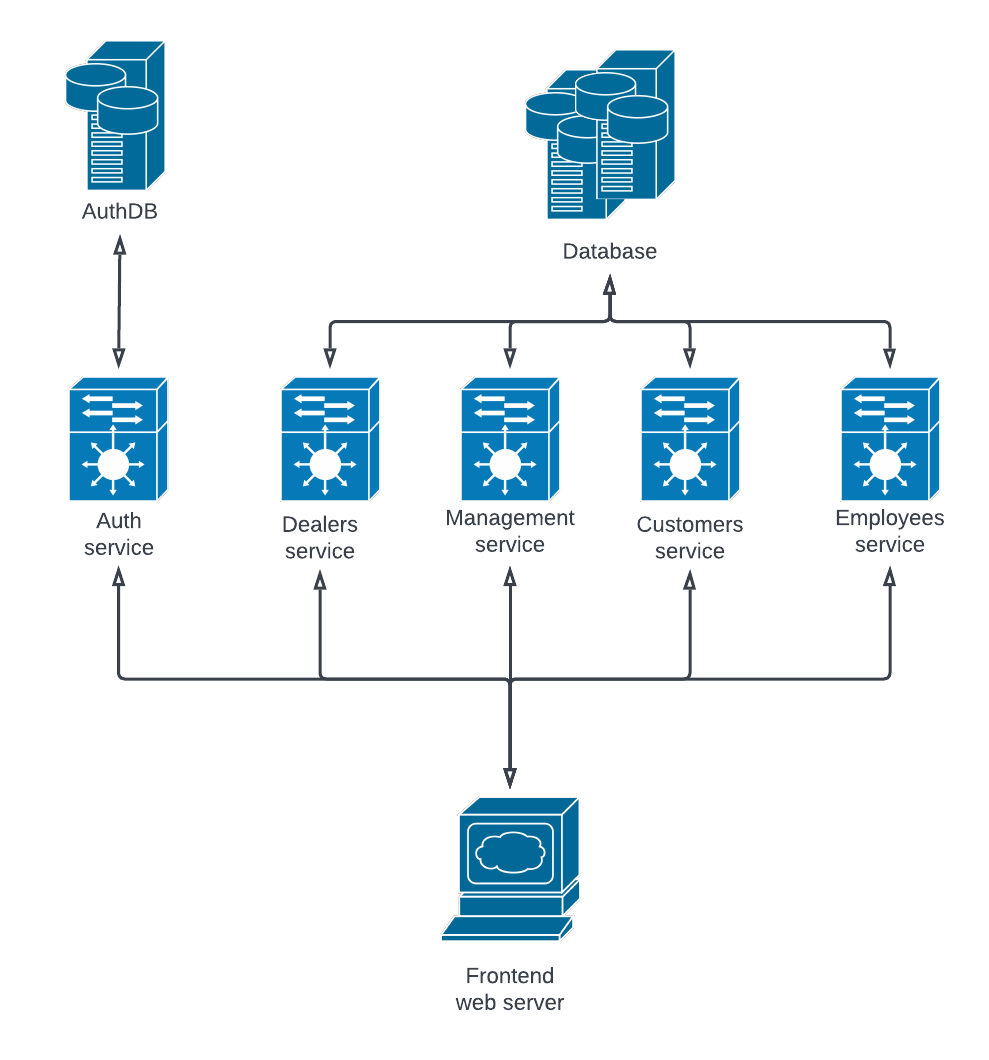
\includegraphics[width=0.9\textwidth]{imgs/arch.png}
    \caption{Architettura}
    \label{fig:arch}
  \end{figure}

  \begin{itemize}
    \item \textbf{Auth service}: servizio che permette di gestire l'autenticazione e 
      l'autorizzazione degli utenti;
    \item \textbf{Dealers service}: servizio che permette di gestire preventivi e ordini;
    \item \textbf{Management service}: servizio che permette di ottenere statistiche e report utili 
      per prendere decisioni strategiche;
    \item \textbf{Customer service}: servizio che permette di gestire le esigenze dei clienti che 
      hanno già acquistato un'auto, come ad esempio: gestione degli appuntamenti ed 
      avvisi di manutenzione obbligatoria;
    \item \textbf{Employees service}: servizio che permette di gestire le ferie e i permessi dei 
      dipendenti;
    \item \textbf{Client frontend}: interfaccia che permette agli utenti di interagire con 
      l'applicativo.
  \end{itemize}

  \subsection{Valore per l'impresa}

  Il valore che l'applicativo porterà all'azienda comprende diversi aspetti:
  \begin{itemize}
    \item \textbf{Automatizzazione dei processi}: l'applicativo permetterà di automatizzare 
      diversi processi interni, permettendo ai dipendenti di concentrarsi su attività più 
      importanti e di valore;
    \item \textbf{Migliore gestione dei clienti}: sarà possibile gestire in modo più efficiente gli appuntamenti
      periodici dei clienti in modo da non congestionare l'officina e migliorare l'esperienza del cliente stesso;
    \item \textbf{Decisioni strategiche}: l'applicativo permetterà ai manager di ottenere statistiche e report, in questo
      modo i manager avranno la possibilità di rilevare e correggere situazioni critiche per l'azienda in modo più tempestivo
      e mirato;
    \item \textbf{Dipendenti}: aumento della soddisfazione dei dipendenti grazie ad una migliore user-experience.
  \end{itemize}


  \subsection{Punti di forza e rischi}
  L'analisi dei rischi approfondita è consultabile nel documento \textcolor{teal}{DealerPro Risk Management}.

  \newpage
  \section{Overview dell'approccio}

  \subsection{Domain Driven Design}

  Si è deciso di utilizzare un approccio di tipo \emph{Domain Driven Design (DDD)} in quanto non si conosceva 
  a fondo il dominio. Sono stati svolti degli incontri preliminari con degli esperti del 
  dominio automobilistico. È stato identificato l’Ubiquitous Language del dominio, il quale verrà utilizzato 
  pervasivamente durante lo sviluppo del progetto. 

  \subsection{Modello PMLC}

  Il modello PMLC scelto rientra nell'ambito dell'Agile Project Management, in particolare si è preferito un  
    approccio iterativo rispetto ad uno adattivo. Questa scelta è stata fatta in quanto il goal del progetto
    è chiaro ma non si riesce ad inquadrare bene la soluzione e le tecnologie potrebbero risultare problematiche.
    Inoltre, lo scope definito in fase di analisi difficilmente subirà cambiamenti data la natura stabile 
    del dominio applicativo. Viste tutte queste motivazioni si è optato per l'approccio
    \emph{Evolutionary Development Waterfall}.
    Il lavoro verrà suddiviso in sprint di durata settimanale.

  \subsection{Attività automatizzabili}

  Sono state identificate tutta una serie di attività che è possibile automatizzare. Questo ha un impatto positivo
  inquanto permette di: ridurre il lavoro del team di sviluppo, ridurre i tempi morti, promuovere l'eccellenza
  tecnica del prodotto e ridurre i rischi di integrazione durante i vari sprint. Queste sono:
  
  \begin{itemize}
    \item \textbf{Testing}: verrà utilizzato un approccio \emph{Test Driven Development (TDD)} per lo sviluppo e
      sarà necessario che tutti questi test diano esito positivo per poter procedere all'integrazione di una nuova
      feature;
    \item \textbf{Gestione del codice}: il codice verrà gestito tramite un sistema di versionamento (Git) e verrà
      utilizzato l'approccio \emph{GitFlow} per la gestione dei branch. Inoltre, i commit saranno scritti seguendo
      la convenzione \emph{Conventional Commits \footnote{\url{https://www.conventionalcommits.org/en/v1.0.0/}}};
    \item \textbf{Versioning}: il versioning del software verrà gestito tramite un sistema di Continuous Integration
      che si occuperà di generare automaticamente un numero di versione incrementale ogni volta che viene 
      effettuato un commit sul branch principale; 
    \item \textbf{Build e deploy}: anche la build e il deploy verranno gestiti tramite un sistema di Continuous 
      Integration che si occuperà di effettuare la build del software e il deploy automatico in un ambiente di testing;
    \item \textbf{Verifica del codice}: prima di poter effettuare un commit il codice verrà controllato da sistemi di 
      linting, verifica di codice duplicato e code coverage. In caso il codice non rispetti i criteri definiti non sarà 
      possibile effettuare il commit su uno dei branch principali ma solo su un branch secondario in attesa di essere
      adattato.
  \end{itemize}

  \newpage
  \section{Riassunto di tempi e risorse}

  \subsection{Stime delle risorse}
  \begin{itemize}
    \item Risorse umane
    \begin{itemize}
      \item 1 Project Manager;
      \item 2 sviluppatori senior;
      \item 2 sviluppatori junior;
      \item 1 graphic designer;
    \end{itemize}
    \item Risorse hardware
    \begin{itemize}
      \item 5 server di produzione (uno per ogni servizio);
      \item 2 database di produzione;
      \item 1 web server di frontend;
      \item 1 server di testing;
      \item 1 database di testing;
    \end{itemize}
    \item Altre risorse
    \begin{itemize}
      \item 1 sala riunioni;
      \item Lavagne;
      \item Pennarelli;
      \item Post-it;
      \item Software grafico per i mock-up;
      \item Software per la gestione dei task del progetto (ad esempio, Trello).
    \end{itemize}
  \end{itemize}

  \subsection{Stime dei tempi}

  Dato il modello PMLC scelto (Evolutionary Development Waterfall) i task sono stati distribuiti secondo sprint
    settimanali. Si è posta particolare attenzione sulle dipendenze tra i vari task e sulla distribuzione delle 
    risorse in modo da non creare conflitti.
    Le risorse sono state redistribuite e/o deallocate durante gli Sprint, al fine di minimizzare i costi 
    ma massimizzare le prestazioni.
    Una prima stima, indicativa, prevede 8 sprint per una durata complessiva di 8 settimane 
    (tuttavia questa stima potrebbe cambiare durante lo svolgimento del progetto). 


\end{document}
